%==============================================================================
%== template for LATEX poster =================================================
%==============================================================================
%
%--A0 beamer slide-------------------------------------------------------------
\documentclass[final]{beamer}
\usepackage[orientation=portrait,size=a0,
            scale=1.25         % font scale factor
           ]{beamerposter}

\geometry{
  hmargin=2.5cm, % little modification of margins
}

%
\usepackage[utf8]{inputenc}

\linespread{1.1}
%
%==The poster style============================================================
\usetheme{sharelatex}

%==Title, date and authors of the poster=======================================
\title
[Final Presentation for ML Course, June 2018, Beijing]
{ % Poster title
AniML : Automatic scoring prediction \\
of Japanese Animation
}


\author{
Valentin KAO and Emile JONAS
}
\institute{Department of Computer Sciences\\
Tsinghua University\\
}
\date{\today}

\begin{document}
\begin{frame}[t]
%==============================================================================
\begin{multicols}{3}
%==============================================================================
%==The poster content==========================================================
%==============================================================================

\section{Introduction}
The Japanese anime industry is a major worldwide success thanks to the interest of other Asian countries. In 2017, the industry pulled in a record \$17.7 billion last year, and boosted by the famous hit, Your Name, growing exports and revenues \cite{web1}. \\
Being able to predict the future smash hits is of great importance in decision making specially in the marketing. In spite of the fact that there are many factors that influence the success of an anime. It is not generally clear how they influence, this project endeavors to determine these factors using machine learning strategies by predicting a score out of 10 based on the data provided by the famous website MyAnimeList. \\

% \structure{Your text with scientific results or something...} $\hat H \Psi = E \Psi$

%\begin{equation}
%H = \sum_{i=1}^{N} h_{D}(i) + \sum_{j>i=1}^{N} C_{ij}
%\end{equation}

%On webpage~\cite{web}
%In Ref.~\cite{ref1}...
%In Refs.~\cite{ref1,ref2}...

\section{Data}

\subsection{Data Collection}
As no adequate dataset existed for this task, we built one, using a Python scraper on MyAnimelist. MyAnimeList is currently the biggest anglophone website about anime. It's a social cataloging application, which means it has both detailed information about anime and a corresponding users aggregated scores. After cleaning, the dataset roughly got 10,000 entries.


\subsection{Data Cleaning and Improvement}
As expected from raw input, a lot of data were incomplete. Either old entries missing information or new entries where the data didn't existed yet. We also removed data that were out of our scope (18+ for example). \\
We replaced non-numerical data by weighted ID. Data values were spread in a really inconsistent way. We used standardization to better fit our algorithm requirement. 

\section{Method}

\subsection{Feature selection}
Currently, the algorithm is using some features like the genre, the date (month and year), weighted related projects, format (episodes/duration), etc. It also use multiple information about users opinion like the total score, how it is spread between values, "favourites", dropped, etc.\\
More complex features (weighted voice actors score, weighted staff score) are to be added in the next versions.
We abandoned features like licensors because they didn't had any beneficial impact on the result. To select (or remove) a features, we determine how correlated the feature is with the others. \\
Moreover, we also used The Recursive Feature Elimination to select the most appropriate features. It uses the model accuracy to identify which attributes (and combination of attributes) contribute the most to predicting the target attribute. \\

\vskip2ex
\begin{figure}
\centering
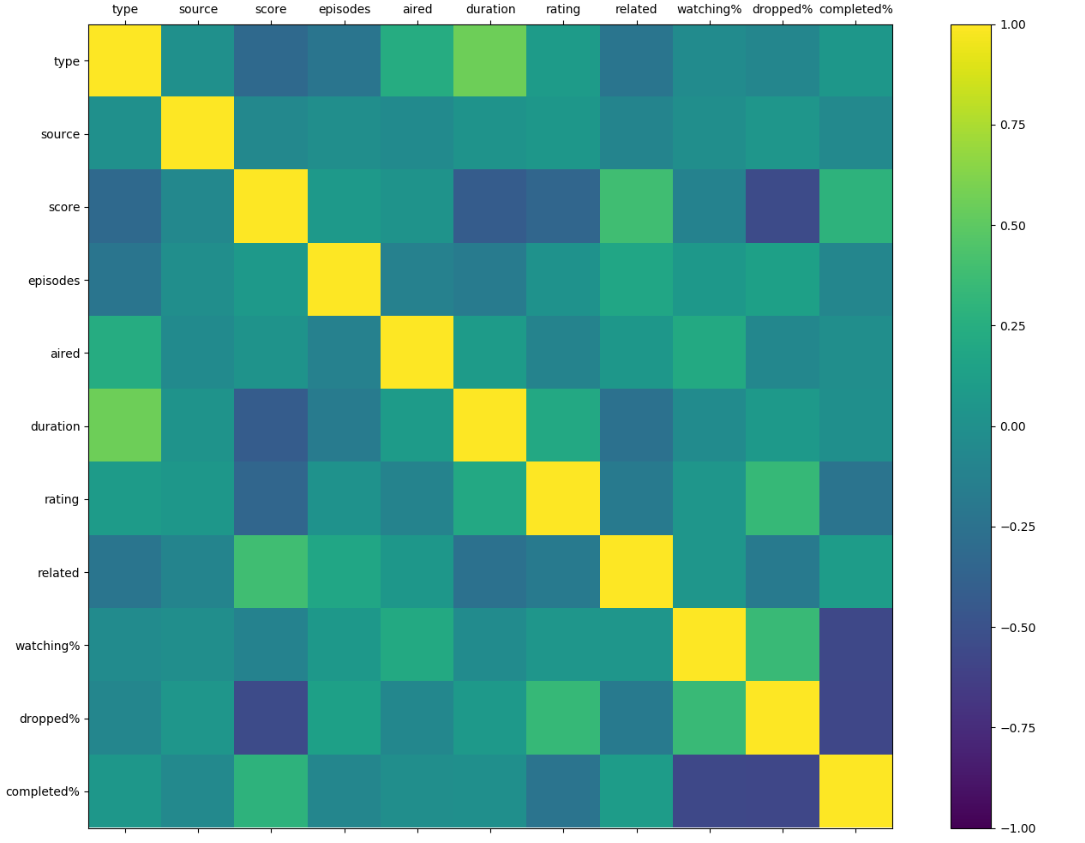
\includegraphics[width=0.9\columnwidth]{corr.png}
\caption{Correlations graph between attributes}
\end{figure}

\subsection{Regression Algorithm Selection}
Since we have small dataset, the selected size of the split of our dataset was 90\% of the data for training and the remaining 10\% for testing. Then, six different algorithm were selected to work on this regression problem. With the default tuning parameters, we performed 3 linear algorithms (Linear Regression, Lasso Regression and ElasticNet) and 3 nonlinear algorithms (Classification and Regression Trees, Support Vector Regression and k-Nearest Neighbors) on our dataset. For evaluating the predictions on these algorithms, we use the Mean Squared Error (or MSE) metric defined by the following formula: \\ \\

\vskip2ex
{\centering \displaystyle \operatorname {MSE} ={\frac {1}{n}}\sum _{i=1}^{n}(Y_{i}-{\hat {Y_{i}}})^{2}.\par}\\
 with \^Y is a vector of n predictions, and Y is the vector of observed values of the variable being predicted.\\
\vskip1ex

\vskip1ex
\begin{figure}
\centering
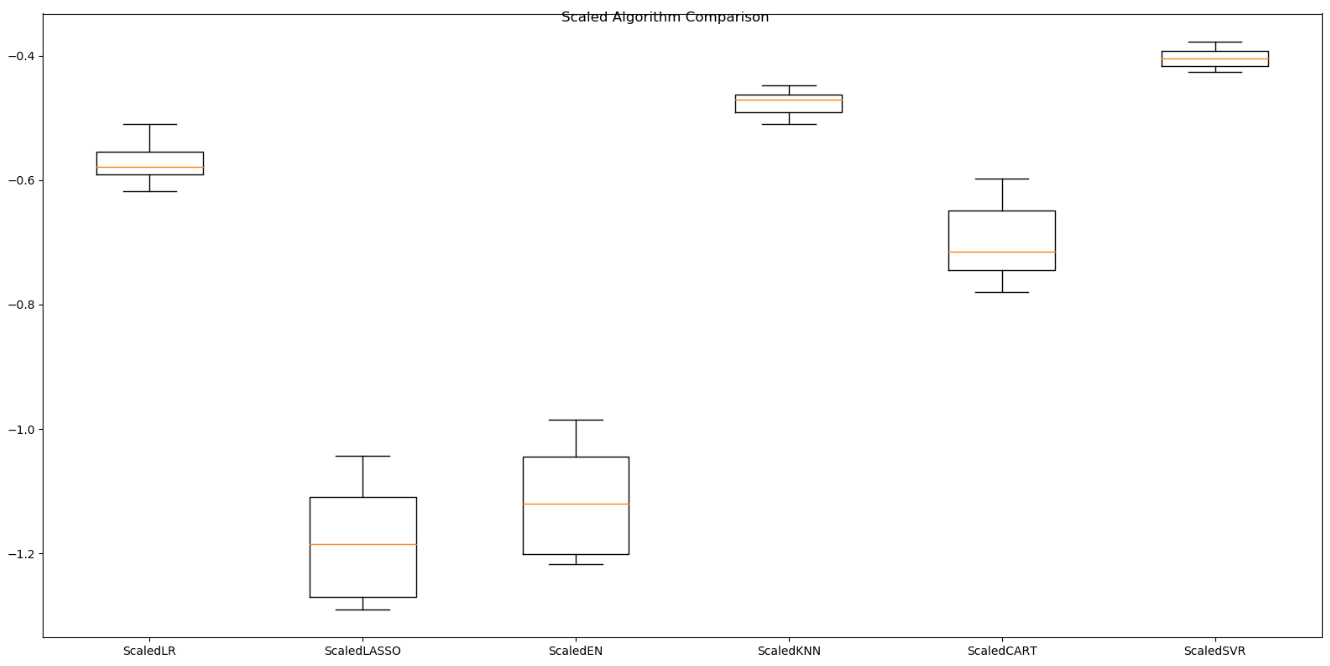
\includegraphics[width=0.99\columnwidth]{plot_regression_algorithm.png}
\caption{Differences in Algorithm Performance on Standardized dataset}
\end{figure}

Then, we can see that Support Vector Regression has both a tight distribution of error and has the lowest score.
To find the most optimal values, we use the Grid search to parameter tuning that will methodically build and evaluate a
model for each combination of algorithm parameters specified in a grid. We obtained the following parameters:

\begin{table}
\centering
\caption{SVR Settings}
\begin{tabular}{ccccc}
\hline\hline   
Parameter & Value\\
\hline
C & 5.0\\
Gamma & '0.1'\\
Kernel & 'rbf'\\
Epsilon & 0.1\\
Tol & 1e-3\\
\hline\hline
\end{tabular}
\end{table}

After implemented the SVR algorithm, we decided to implement an ensemble method.  We evaluated four different ensemble machine learning
algorithms, two boosting and two bagging methods. 

\vskip2ex
\begin{figure}
\centering
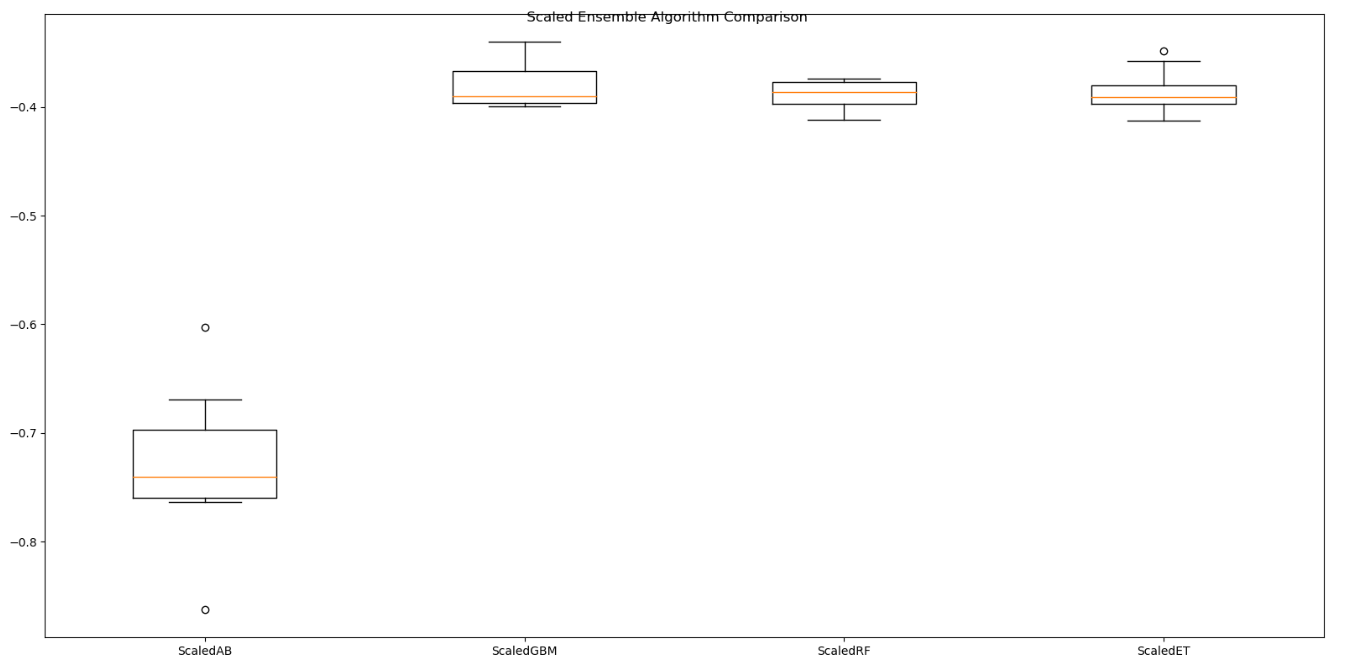
\includegraphics[width=0.99\columnwidth]{plot_ensemble_algorithms.png}
\caption{Differences in Ensemble Algorithm Performance on  dataset}
\end{figure}

According to the statistics, the scores are better than the linear and nonlinear algorithms. We decided to tune the Gradiant Boosting algorithm since its MSE is the lowest, and also, the Extra Tree Regressor algorithm since its derivation is the lowest. As well as the SVR algorithm tuning, we use Grid Search method to obtain the following parameters.\\

\vskip2ex
\begin{table}
\centering
\caption{Ensemble Algorithm Settings}
\begin{tabular}{ccccc}
\hline\hline\hline
GBM & & ET \\
\hline\hline
Parameter & Value & Parameter & Value \\
min samples leaf & 1 & learning rate & 0.1 \\
min samples split & 6 & max depth & 7.0 \\
n estimators & 725 & n estimators & 600 \\
\hline\hline
\end{tabular}
\end{table}
\vskip2ex

\section{Results}

\vskip1ex
\begin{table}
\centering
\caption{Results from tuned algorithm.}
\begin{tabular}{ccccc}
\hline\hline   
Algorithm & Mean Squared Error\\
\hline
SVR & 0.42640\\
Gradiant Boosting & 0.33878\\
Extra Trees & 0.38938\\
\hline\hline
\end{tabular}
\end{table}
\vskip2ex

After having tuned our three algorithms, we calculated the final Mean Squared Error of each algorithm. We can see that the best score we have is from the Gradiant Boosting Algorithm. The mean squared error is 0.33878 meaning that in average, meaning that we have an error of 0.57 on the score out of 10, for any anime. \\

\subsection{Amelioration}
The current size of the dataset is really small, we hope to obtain the last 20,000 for the final report. Moreover, the features selected are based on numbers and identifiants without taking into account the title and the synopsis of the anime. A huge amelioration would be using the title and the synopsis as features, by analyzing the words containing.\\

\section{Summary and conclusions}
This project imagined by ourselves is a regression predictive modeling machine learning problem. By computing multiple linear, nonlinear and ensemble algorithms on a self-made dataset built from scratch, we finally predict with a error margin of 5.7\% the score of a anime.\\

%==============================================================================
%==End of content==============================================================
%==============================================================================

%--References------------------------------------------------------------------

\subsection{References}

\begin{thebibliography}{99}

\bibitem{web1} \textit{Rafael Antonio Pineda (2017, October). "Anime Industry Takes in Record 2.0 Trillion Yen in 2016" retrieved 4th june of 2018 from} \url{https://www.animenewsnetwork.com/news/2017-10-25/anime-industry-takes-in-record-2.0-trillion-yen-in-2016/.123164}

\bibitem{web2} \textit{MyAnimeList website} \url{https://myanimelist.net/}

\end{thebibliography}
\vskip2ex
%--End of references-----------------------------------------------------------

\end{multicols}

\end{frame}

\end{document}
